\cftinserthook{toc}{backmattertoc}
\backmatter
%\markboth{}{} %clear the header marks
\appendix
\cleartorecto
\appendixpage
%\addappheadtotoc
\onecolumn
\setcounter{footnote}{0}
\chapter*{Apocalyptic Numbers}
%\markboth{Apocalyptic Numbers}{}
\fancyhead{} %clear formatting
\fancyhead[LE]{APPENDICES} %for even pages, put the chapter number on left side; for odd pages, put chapter title on right
\fancyhead[RO]{APOCALYPTIC NUMBERS}
\addcontentsline{toc}{section}{Apocalyptic Numbers}

When Christ revealed the apocalyptic vision to John, he did so in a way that made sense in light of previous 
apocalyptic visions seen by prophets like Daniel, Ezekiel, Zechariah and others. One feature of the apocalyptic 
tradition is the deliberate use of symbolic numbers like one, two, three, four, six, seven, and twelve, along with their multiples. 
John, like previous seers, does not often explain the symbolism of these numbers; it is the audience's 
responsibility to study the entire body of inspired Scripture and to make the mental connections. 
\newline\newline
The study of biblical numbers is fraught with danger; many have gone beyond what can be scripturally supported in search of hidden messages in the text and in the wider world%
\footnote{Some, combining pagan spiritualist beliefs with Scripture, claim that seeing certain numbers like 777 repeated in one's environment (license plates, phone numbers, etc.) is a sure sign of guidance from guardian angels. This doctrine of ``angel numbers'' is nowhere found in Scripture. Others have applied Chaldean numerology to biblical genealogies and other texts seeking to tease out hidden messages. This, too, is vanity.}%
. In this, as in all biblical studies, may the text and not our imagination be the guide. The other extreme would be to completely ignore the biblical tradition of using numbers symbolically. This has led some to propose, for example, that the number 144,000 should be read at face value as the exact number of those who will be resurrected to heaven. This unstudied interpretation ignores the wider apocalyptic use of the number 12 and its multiples, presents insurmountable obstacles to a unified interpretation of John's vision%
\footnote{If the 144,000 figure is taken literally, a consistent approach would also take the tribal counts literally in 7:5-8, but few do so for obvious historical reasons.} %
and ultimately leads to major doctrinal error.
\newline\newline
Instead of either of these extremes, the most sure path is to interpret the different numbers in Revelation in light of the entire body of Scripture. A solid background knowledge of the Bible will lead readers of Revelation to appreciate the rich tradition behind the different numbers and guide them to better interpretation. The numbers do not encode mystical messages discernible only to the initiated. They are readily intelligible to biblically informed Christians and offer yet another way the Spirit enriches his faith-producing message to us. 
\newline\newline
To offer a secular comparison, this is similar to the way the American flag is meaningful to US citizens in part because of the number of stars and stripes on it. It is not that the flag is encoding a secret message; rather, for those who have studied American history and understand the national significance of the numbers 13 and 50, the flag is able to say much without having a single word written on it. So, John and other apocalyptic authors are able to import freight loads of symbolic meaning into their written messages without having to explicitly rehash previous biblical texts. Using these numbers is a kind of inspired shorthand which is meaningful to citizens of the kingdom of heaven.
\newline\newline
The tables presented below make an attempt to provide some scriptural background for the use of different numbers in Revelation. It is essential to note that not every number in the apocalyptic literature fits neatly into the categories laid out here. Many do not and it is up to each Bible student to draw their own conclusions.

\section*{One}

In Revelation, as in the rest of the Bible, God reveals himself to us as One without comparison. Of course, not every instance of the word ``one'' is meant to point toward Deity (for example, in the \textsc{ASV} see 1:17; 2:17); but a few do - Christ is the Living One (1:18), there is One sitting upon the throne (4:2), and God is the Holy One (16:5).
\newline\newline
\definecolor{headergray}{HTML}{ECECEC}
\definecolor{lightgray}{HTML}{F5F5F5}
\definecolor{lightergray}{HTML}{FAFAFA}
\rowcolors{3}{lightgray}{lightergray}
\begin{tabularx}{\textwidth}{l X}
\toprule
\rowcolor{headergray}\emph{Reference} & \emph{Information}\\ 
\midrule
Deuteronomy 6:4 & ``Hear, O Israel: Jehovah our God is one Jehovah'' \\
\addlinespace
John 10:30 & ``I and the Father are one'' \\
\bottomrule
\end{tabularx}
	
\section*{Two}
The most memorable pair in Revelation are God's two witnesses who ``are the two olive trees and the two candlesticks'' (11:3-4). God commanded in Deuteronomy 19.15 that all accusations be confirmed by a minimum of two witnesses and the two witnesses of the Apocalypse follow the example of other pairs of God's messengers like the two angels who were sent to Sodom to warn Lot of the coming destruction (Genesis 19:1). Jesus also sent his disciples out in pairs (Mark 6:7) and great power was granted to any two disciples who agreed on a heavenly petition - the Father would fulfil it and Christ would be in their midst (Matthew 18:19-20).  
\newline\newline
\begin{tabularx}{\textwidth}{l X}
\toprule
\rowcolor{headergray}\emph{Reference} & \emph{Information}\\ 
\midrule
Genesis 19:1 & ``The two angels came to Sodom at even\ldots'' \\
\addlinespace
Deuteronomy 19:15 & ``One witness shall not rise up against a man for any iniquity, or for any sin, in any sin that he sinneth: at the mouth of two witnesses, or at the mouth of three witnesses, shall a matter be established.'' \\
\addlinespace
Matthew 18:16-20 & ``If he hear thee not, take with thee one or two more, that at the mouth of two witnesses or three every word may be established\ldots~ if two of you shall agree on earth as touching anything that they shall ask, it shall be done for them of my Father who is in heaven. For where two or three are gathered together in my name, there am I in the midst of them'' \\
\addlinespace
Mark 6:7 & ``He calleth unto him the twelve, and began to send them forth by two and two; and he gave them authority over the unclean spirits.'' \\
\bottomrule
\end{tabularx}

\section*{Three}
The book of Revelation makes frequent use of threes, starting as early as 1.2, where John claims to bear witness to (1) the word of God, (2) the testimony of Jesus and (3) all things that he saw. The Triune God is given a full introduction in 1.4-5 and within that introduction are two other descriptive triplets: the Father is described as he who (1) is, (2) was and (3) is to come and Christ is described as (1) faithful witness, (2) firstborn from the dead and (3) ruler of kings. Later in the vision and standing in contrast to the holy Trinity is a diabolical trinity composed of the dragon, the beast and the false prophet (16:13). These three send out three frog-like unclean spirits to gather the nations for Armaggedon.
\newline\newline
Elsewhere in the Scriptures, the number three is sometimes associated with completeness or perfection. Previous to the New Testament's trinitarian statements, there are several well-known Old Testament triplets like the three patriarchs, Daniel's three friends, the seraph's cry of ``Holy, holy, holy''. The Old Testament itself is divided into three: ``the law of Moses, and the prophets, and the psalms'' (Luke 24:44). The New Testament more strongly connects three with the concept of wholeness or perfection.  
\newline\newline
\begin{tabularx}{\textwidth}{l X}
\toprule
\rowcolor{headergray}\emph{Reference} & \emph{Information}\\ 
\midrule
Isaiah 6:3 & ``One cried unto another, and said, Holy, holy, holy, is Jehovah of hosts\ldots'' \\
\addlinespace
Matthew 28:19 & ``Go ye therefore, and make disciples of all the nations, baptizing them into the name of the Father and of the Son and of the Holy Spirit'' \\
\addlinespace
Luke 1:35 &  ``The Holy Spirit shall come upon thee, and the power of the Most High shall overshadow thee: wherefore also the holy thing which is begotten shall be called the Son of God'' \\
\addlinespace
Luke 24:44 & ``All things must needs be fulfilled, which are written in the law of Moses, and the prophets, and the psalms, concerning me'' \\
\addlinespace
2 Corinthians 13:14 & ``The grace of the Lord Jesus Christ, and the love of God, and the communion of the Holy Spirit, be with you all'' \\
\addlinespace
1 Peter 1:2 & ``According to the foreknowledge of God the Father, in sanctification of the Spirit, unto obedience and sprinkling of the blood of Jesus Christ'' \\
\bottomrule
\end{tabularx}

\section*{Four}
In Revelation, as in Ezekiel, there are four living creatures around the throne of God (4:6; cf. Ezekiel 1:4-28). In Ezekiel, the spirit of these living beings is in four wheels which go in four directions upon the earth. This indicates that the number four is often, though not always, related to the earth with its four cardinal directions.
Elsewhere in Revelation, there are four angels at the four corners of the earth holding back the four winds of the earth (7:1) and Satan deceives the nations in the four corners of the earth (20:8). 
\newline\newline
One other interesting use of the number four relates to the days of creation. God created the sun, moon and stars on the fourth day (Genesis 1:14-19) and in John's vision, the fourth trumpet darkens a third of the heavenly host (8:12), while the fourth bowl of wrath is poured out on the sun, provoking scorching heat (16:8). It is as though the fourth trumpet and the fourth bowl are reminding humanity that God is still more than capable of controlling today those heavenly bodies he created on the fourth day.
\newline\newline
\begin{tabularx}{\textwidth}{l X}
\toprule
\rowcolor{headergray}\emph{Reference} & \emph{Information}\\ 
\midrule
Genesis 1:14-19 & ``God made the two great lights; the greater light to rule the day, and the lesser light to rule the night: he made the stars also\ldots~ And there was evening and there was morning, a fourth day'' \\
\addlinespace
Isaiah 11:12 & ``And he will set up an ensign for the nations, and will assemble the outcasts of Israel, and gather together the dispersed of Judah from the four corners of the earth.'' \\
\addlinespace
Ezekiel 7:2 & ``Thus saith the Lord Jehovah unto the land of Israel, An end: the end is come upon the four corners of the land.'' \\
\bottomrule
\end{tabularx}

\section*{Six}
While much has been made of the number six and especially 666, the number is actually mentioned very few times in Revelation. The four living creatures have six wings in John's vision (4:8) like the seraphim of Isaiah's vision (6:2), as opposed to four as in Ezekiel (1:6). It is difficult to determine what might be the reason for this change other than to evoke connections at once with both Isaiah and Ezekiel's visions.
\newline\newline
Then of course there is the number of the beast, which ``is the number of a man'': 666 (13:18). There are some manuscripts which read 616, but the prevailing consensus is that 666 is the best reading. What this number means has been debated \textit{ad infinitum}; perhaps it refers to the sum of the letters of Nero Caesar or perhaps it is a deliberate repitition of the number six, the day on which man was created (Genesis 1:24-31). It could be something else entirely. Here, as always, it is up to the Bible student to show diligence in coming to his or her own conclusions.
\newline\newline
\begin{tabularx}{\textwidth}{l X}
\toprule
\rowcolor{headergray}\emph{Reference} & \emph{Information}\\ 
\midrule
Genesis 1:24-31 & ``God created man in his own image, in the image of God created he him; male and female created he them\ldots~ And there was evening and there was morning, the sixth day.'' \\
\bottomrule
\end{tabularx}

\section*{Seven}
John's vision, like his gospel account,%
	\footnote{Seven signs (turning water to wine, healing the nobleman's son, healing the lame man, feeding the 5,000, walking on water, healing the blind man, raising Lazarus), seven ``I am'' statements (``bread of life'', ``light of the world'', ``door'', ``good shepherd'', ``resurrection and the life'', ``way, the truth and the life'', ``true vine''), seven disciples mentioned in 21:2, etc.} %
is loaded with references to the number seven. It is addressed to seven churches represented by seven golden candlesticks (1:4, 11, 12, 20). There are seven stars in Christ's right hand representing the seven angels of the churches (1:16, 20). There are seven spirits before the throne of God (1:4; 4:5). There are seven seals on the scroll in God's right hand (5:1). Christ appears as a lamb with seven horns and seven eyes which are the seven spirits of God (5:6). Once the seventh seal is broken, seven angels sound seven trumpets (8:1-2). When a mighty voice roars, seven thunders utter their voices (10:3-4). An earthquake kills 7,000 people (11:13). The great red dragon has seven heads and seven diadems (12:3). Later come seven more angels with the seven bowls of wrath (15:1). The great harlot rides upon a beast with seven heads, representing seven mountains upon which the harlot sits; they also represent seven kings (17:3, 7, 9-11). 
\newline\newline
Certain key words in Revelation appear in multiples of seven:%
	\footnote{Peter Williamson. \textit{Revelation}. Baker Academic, 2015.} %
\begin{itemize}
 \item ``Lord God Almighty'' occurs seven times (1:8; 4:8; 11:17; 15:3; 16:7; 19:6; 21:22)
 \item ``Christ'' seven times (1:1, 2, 5; 11:15; 12:10; 20:4, 6)
 \item ``Jesus'' 14 times (1:1, 2, 5, 9 [2x]; 12:17; 14:12; 17:6; 19:10 [2x]; 20:4; 22:16, 20, 21)
 \item ``Lamb''  28 times\footnote{13:11 is not counted since it refers to the land beast}
\end{itemize}
John may have deliberately avoided using other words in multiples of seven:
\begin{itemize}
\item ``Satan'' occurs eight times (2:9, 13 [2x], 24; 3:9; 12:9; 20:2, 7)
\item ``dragon'' 13 times (12:3, 4, 7 [2x], 9, 13, 16, 17; 13:2, 4, 11; 16:13; 20:2)
\item ``Babylon'' six times (14:8; 16:19; 17:5; 18:2, 10, 21)
\end{itemize}
From the beginning, the number seven has been symbolic of perfection or completion. The very first verse of the Bible is composed of seven words and 28 (a multiple of 7) letters in Hebrew. The second verse is 14 words in Hebrew.  God rested from creation on the seventh day. The description of that seventh day in Genesis 2.1-3 has 35 words.%
	\footnote{Goodfriend, E. (2021). \textit{Seven, the Biblical Number}. TheTorah.com. https://thetorah.com/article/seven-the-biblical-number\label{torah_seven}} %
Seven times in Genesis 1, God saw that his creation was good. God protected Cain by warning that any who killed him would pay a sevenfold vengeance. Lamech, the seventh man starting with Adam and going through Cain, says he will be avenged seventy-sevenfold. Enoch, the seventh man starting with Adam and going through Seth, did not see death since God took him. Jacob served Laban 7 years for Rachel. He bowed seven times before his brother Esau. Seventy souls of Jacob's family moved to Egypt. There are too many other sevens in the Bible to mention here.  
\newline\newline
\begin{tabularx}{\textwidth}{l X}
\toprule
\rowcolor{headergray}\emph{Reference} & \emph{Information}\\ 
\midrule
Genesis 1:1 & The verse contains 7 words and 28 letters in Hebrew\footref{torah_seven} \\
\addlinespace
Genesis 1:2 & The verse contains 14 words in Hebrew\footnote{Ibid.\label{ibid}} \\
\addlinespace
Genesis 1:4, 10, 12, 18, 21, 25, 31 & God saw that His creation was good 7 times \\
\addlinespace
Genesis 1:1-2:3 & 6 Days of Creation + Sabbath day\\
\addlinespace
Genesis 2:1-3 & The description of the seventh day has 35 words in Hebrew\footref{ibid} \\
\addlinespace
Genesis 4:24 & ``If Cain shall be avenged sevenfold, truly Lamech [seventh generation] seventy and sevenfold'' \\
\addlinespace
Genesis 5:24 & ``Enoch [seventh generation] walked with God: and he was not; for God took him.'' \\
\addlinespace
Genesis 29:18, 20 & ``Jacob served seven years for Rachel'' \\
\addlinespace
Genesis 33:3 & ``He himself passed over before them, and bowed himself to the ground seven times, until he came near to his brother'' \\
\addlinespace
Exodus 1:5 & ``All the souls that came out of the loins of Jacob were seventy souls'' \\
\bottomrule
\end{tabularx}

\section*{Twelve}
John saw 24 elders before God's throne. There were 12,000 individuals sealed from each of twelve tribes of Israel (7:4-8). The woman arrayed with the sun wears a crown of twelve stars (12:1). The new Jerusalem has twelve gates, twelve foundations and is twelve thousand furlongs square (21:12, 14, 16). The tree of life bears twelve types of fruits, bearing fruit each month (22:2). 
\newline\newline
Beginning with the twelve sons of Jacob and then with the twelve landed tribes of Israel,%
\footnote{Joshua 13-19} %
the number twelve came to symbolize God's chosen people. Jesus' choosing of twelve disciples appears to have been at least partly based on this: ``Ye also shall sit upon twelve thrones, judging the twelve tribes of Israel'' (Matthew 19:28). 
\newline\newline
It can be safely assumed that when these sets of twelve are mentioned, God is pointing to the idea of his special people, his chosen community.
\newline\newline
\begin{tabularx}{\textwidth}{l X}
\toprule
\rowcolor{headergray}\emph{Reference} & \emph{Information}\\ 
\midrule
Genesis 35:22; Exodus 39:14; Ezekiel 47:13 & Twelve sons or tribes of Israel \\
\addlinespace
Matthew 10:1-2; 19:28 & Twelve apostles of Christ \\
\bottomrule
\end{tabularx}

\printindex[gen]
\chapter{Notes}
\fancyhead{} %clear formatting
\fancyhead[LE]{NOTES} %for even pages, put the chapter number on left side; for odd pages, put chapter title on right
\fancyhead[RO]{NOTES}
\newpage\mbox{}\cleardoublepage
\newpage\mbox{}\cleardoublepage
\renewcommand*{\BRbooktitlestyle}[1]{\textbf{#1}\nopagebreak}
\clearpage
\chaptermark{Scripture Index}
\fancyhead{} %clear formatting
\fancyhead[LE]{SCRIPTURE INDEX} %for even pages, put the chapter number on left side; for odd pages, put chapter title on right
\fancyhead[RO]{SCRIPTURE INDEX}
\printindex[scr]

%maps
\cleartoverso
\pagestyle{plain}
%\captionsetup[figure]{labelformat=empty}

\begin{sidewaysfigure}
    \centering
    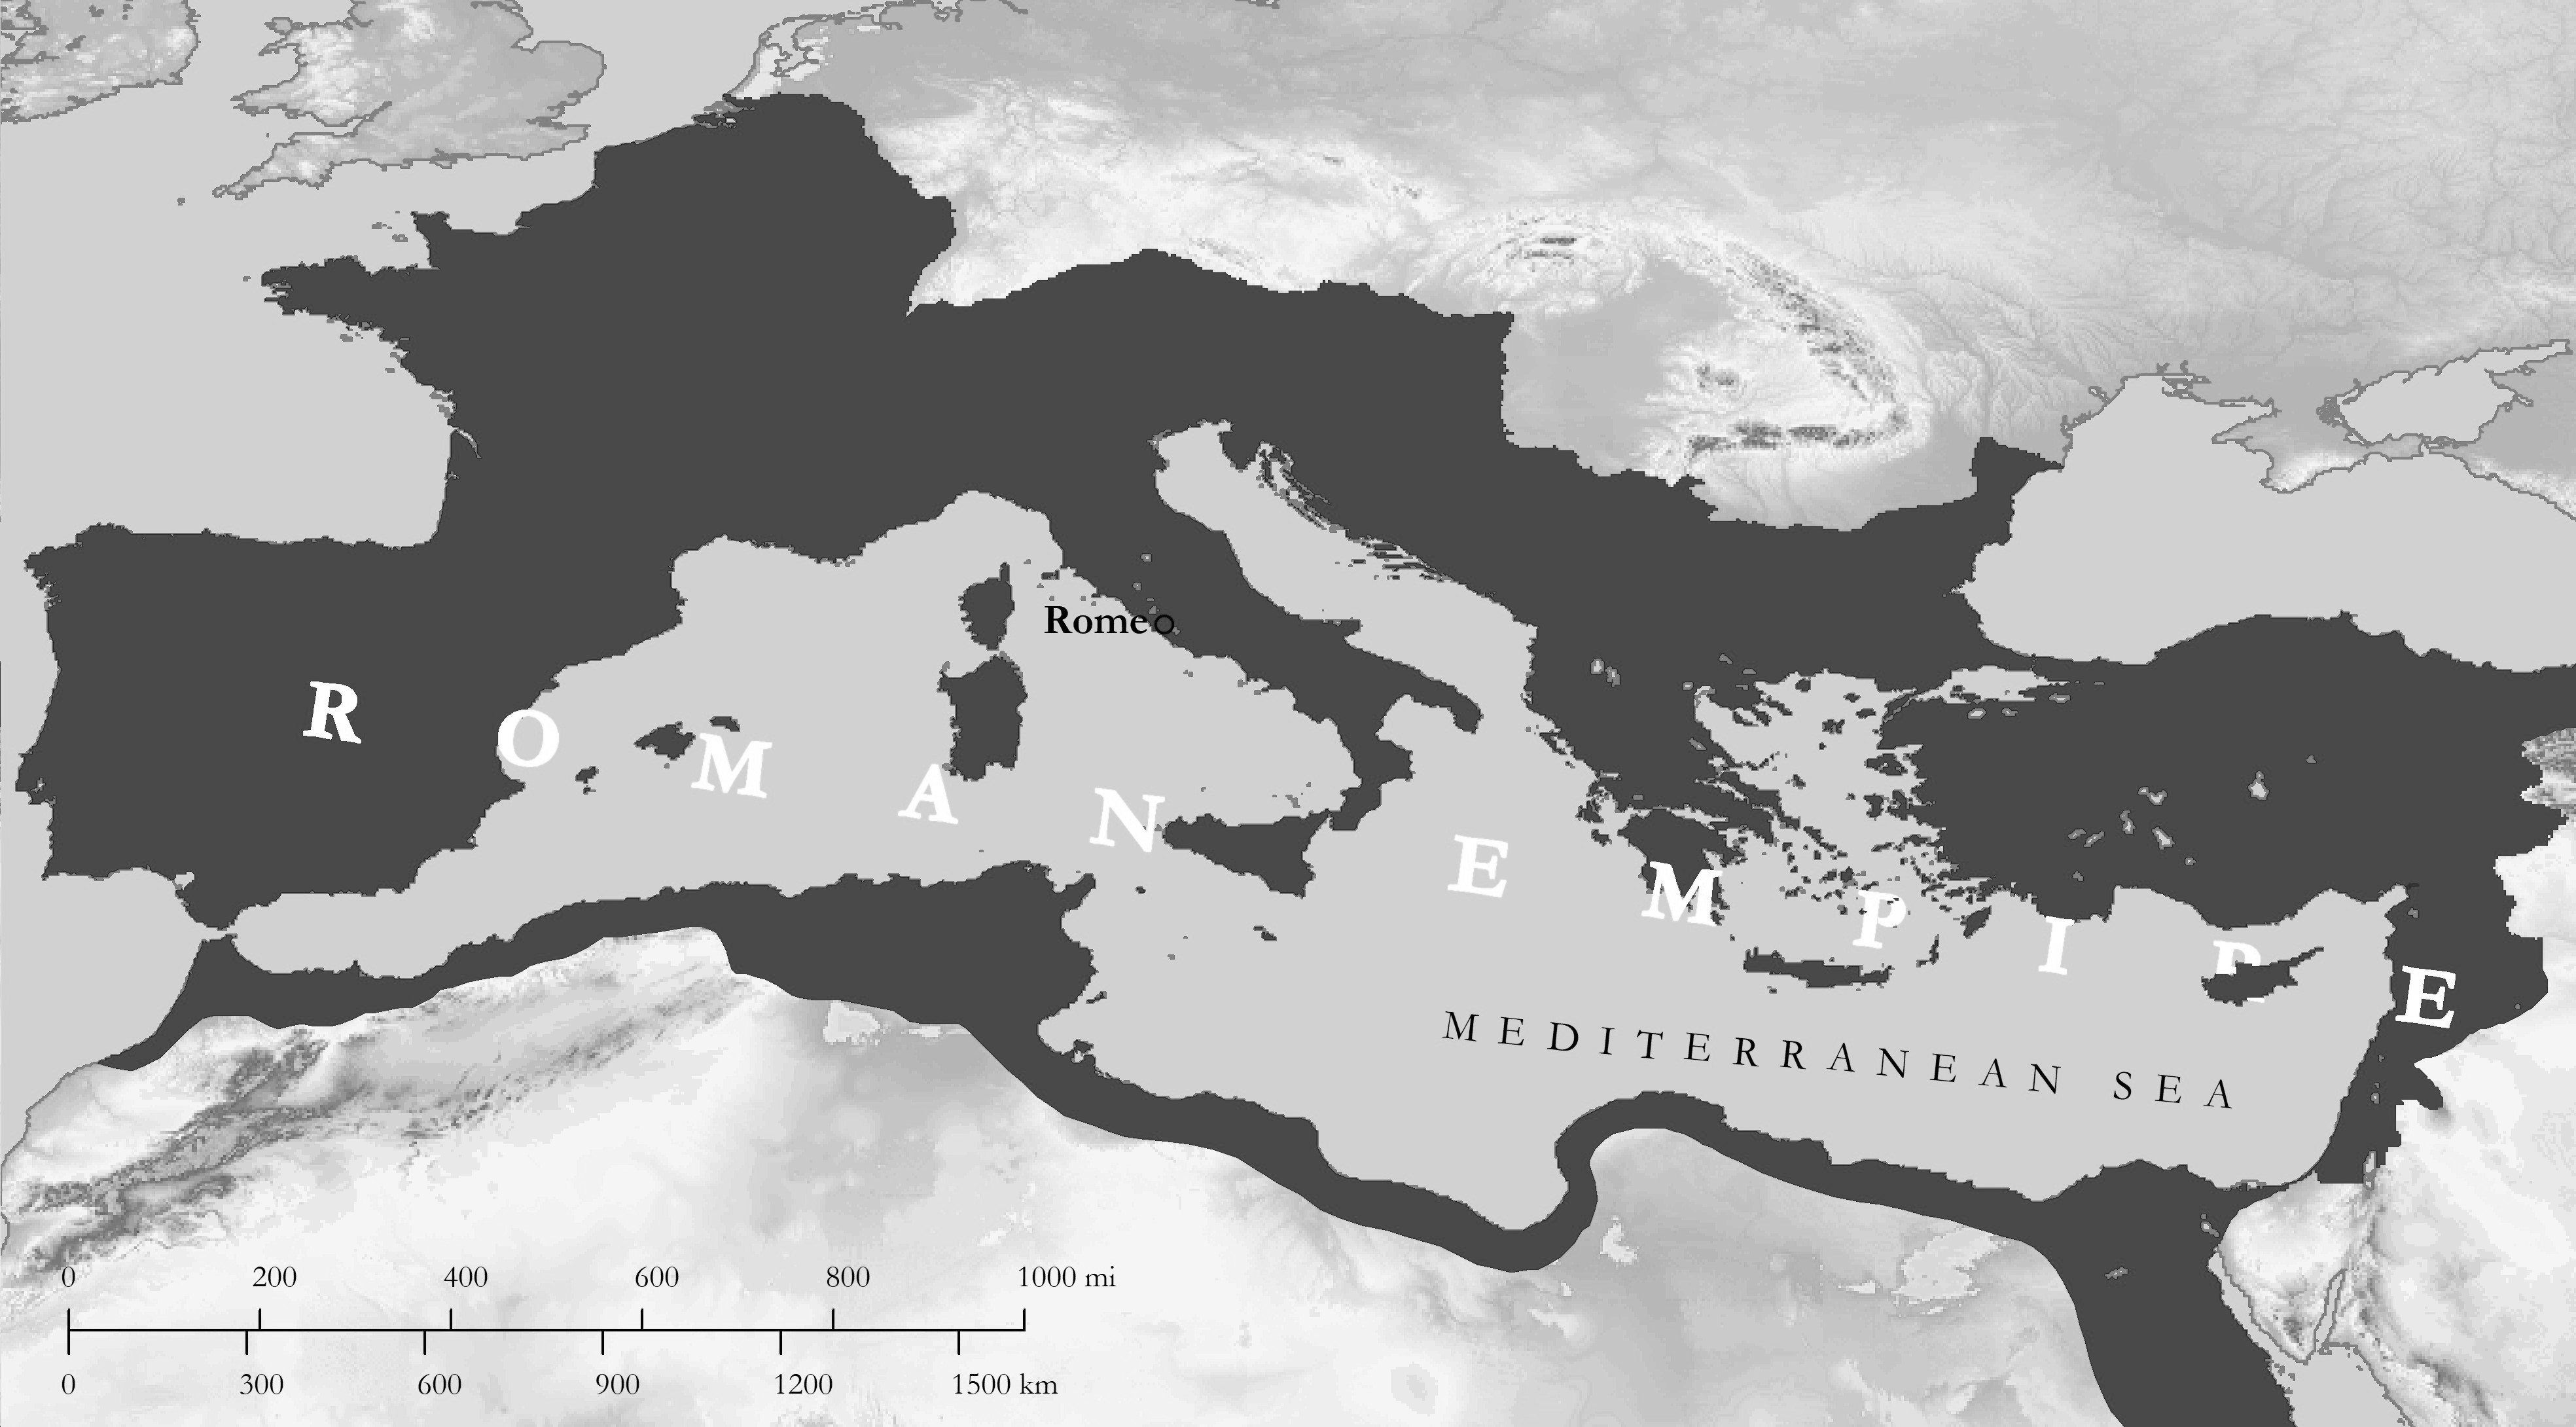
\includegraphics[width=\paperwidth,height=0.9\paperheight,keepaspectratio]{images/romanempire_bw.jpg}
\end{sidewaysfigure}

\begin{sidewaysfigure}
    \centering
    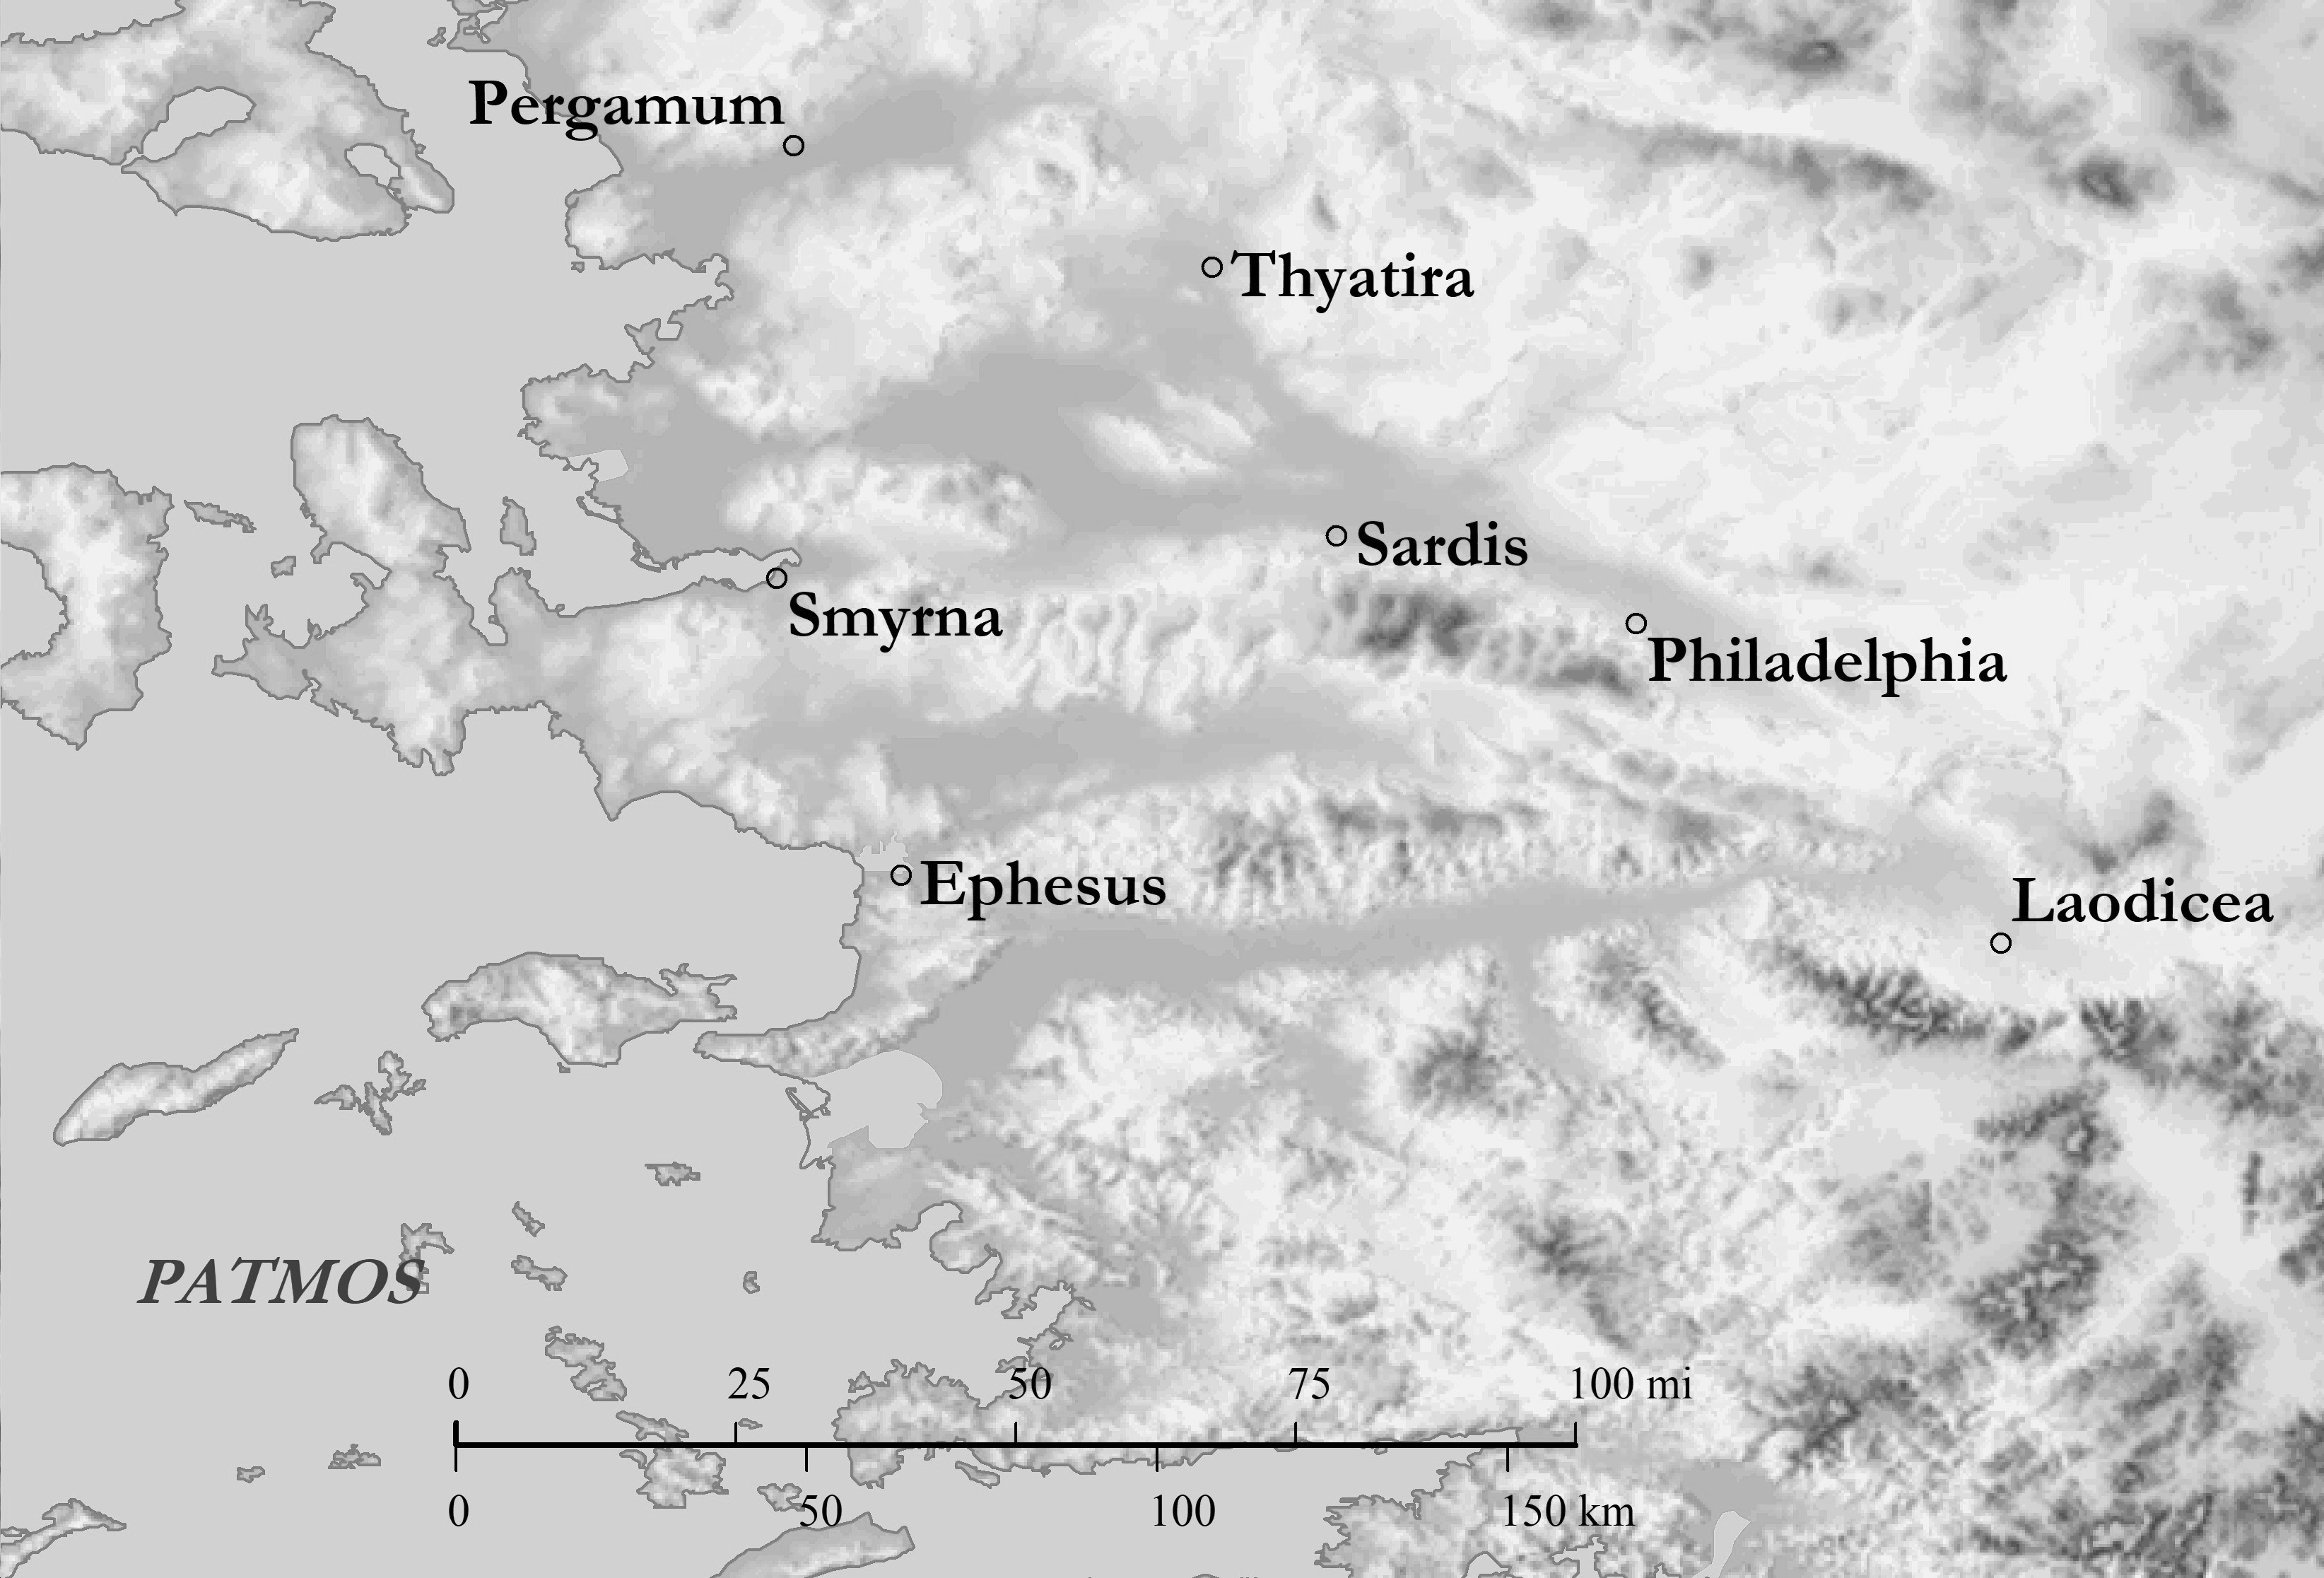
\includegraphics[width=\paperwidth,height=0.9\paperheight,keepaspectratio]{images/sevenchurches_bw.jpg}
\end{sidewaysfigure}